\chapter{}
\section{Вступні відомості}
\noindent\textbf{Мета роботи:} Ознайомлення з принципами баєсівського підходу в криптоаналізі, побудова детерміністичної та стохастичної 
вирішуючих функцій для моделей схем шифрування та криптоаналіз моделей шифрів за допомогою програмної реалізації, зокрема здійснення 
порвіняльного аналізу вирішуючих функцій.

\noindent\textbf{Постановка задачі:}
\begin{enumerate}
    \item Створіть репозиторій у системі контролю версій Git/GitHub;
    \item Реалізуйте алгоритми програмно та представите результати побудови детермінованих та стохастичних вирішальних функцій у 
        вигляді таблиць. Для цього необхідно:
        \begin{enumerate}
            \item обчислити розподіли $P(C)$ та $P(M, C)$;
            \item на основі цих розподілів обчислити $P(M \vert C)$;
            \item побудова оптимальних детермінованих та стохастичних вирішальних функцій зводиться до максимізації $P(M \vert C)$.
        \end{enumerate}
    \item Розрахуйте середні втрати, проведіть порівняльний аналіз функцій прийняття рішень.
    \item Підготувати звіт для комп'ютерного практикуму.
\end{enumerate}
\section{Результати виконання роботи. Варіант 15}
$P (C_{k}) = \sum\limits_{i, j : (i, j) = k} P(M_{i}) \cdot P(K_{j})$
\begin{figure}[!ht]
    \centering
    \begin{minipage}{0.6\linewidth}
        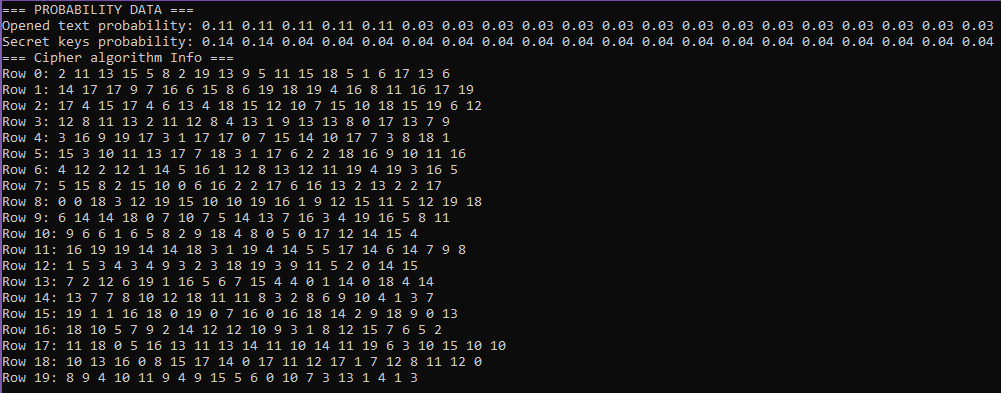
\includegraphics[width=0.6\textwidth, scale=0.05]{ReportPic/report_1.png}
    \end{minipage}
\end{figure}
\newpage
\begin{figure}[!ht]
    \centering
    \begin{minipage}{0.35\linewidth}
        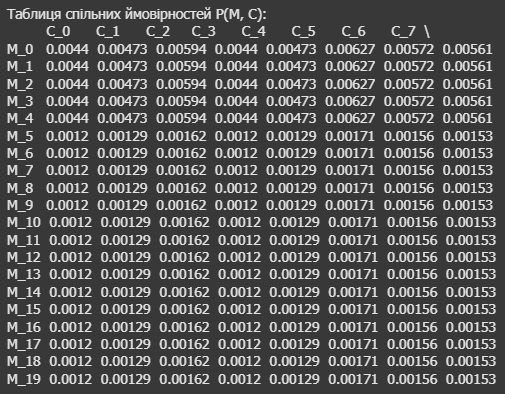
\includegraphics[width=0.85\textwidth]{ReportPic/report_2.1.png}
    \end{minipage}
    \begin{minipage}{0.35\linewidth}
        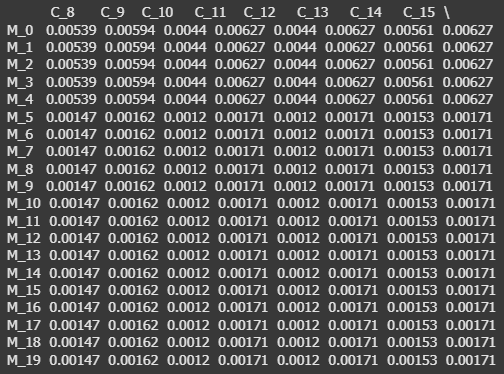
\includegraphics[width=0.85\textwidth]{ReportPic/report_2.2.png}
    \end{minipage}
    \begin{minipage}{0.25\linewidth}
        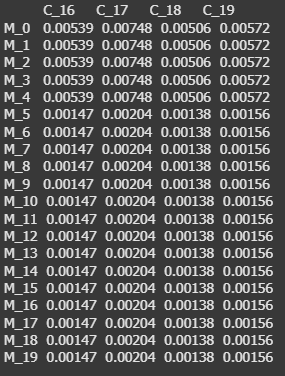
\includegraphics[width=0.85\textwidth]{ReportPic/report_2.3.png}
    \end{minipage}
\end{figure}
\begin{figure}[!ht]
        \centering
        \begin{minipage}{0.55\linewidth}
            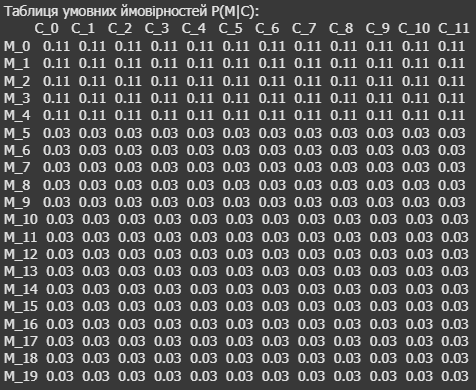
\includegraphics[width=0.8\textwidth, scale=0.6]{ReportPic/report_3.1.png}
        \end{minipage}
        \begin{minipage}{0.4\linewidth}
            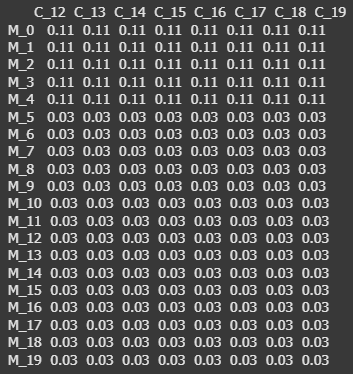
\includegraphics[width=0.8\textwidth, scale=0.5]{ReportPic/report_3.2.png}
        \end{minipage}
\end{figure}
\section{Побудова вирішуючих функцій}
\begin{definition}    
    ~\par Оптимальна (баєсівська) детерміністична функція [в межах лабораторної роботи] визначається наступним чином: 
    \begin{equation*}
        \delta_{B} = \left\{\delta_{B}^{(n)} : \mathcal{M} \rightarrow \mathcal{C}\right\}, 
    \end{equation*}
    де $P \left(\delta_{B}^{(optim)} \vert C\right) = \max\limits_{m \in M} P \left(M_{i} \vert C\right)$. \\ 
    Тобто фактично детерміністична функція дорівнює довільному шифротексту, який дорівнює максимальному значенню в 
    $i$-тому рядку таблиці.
\end{definition}
\begin{definition}
    ~\par Стохастична розв'язувальна функція $\delta_{D}$ є оптимальною тоді і тільки тоді, коли $\forall \, n$ 
    з нерівності $\delta_{c}^{(n)} \left(C, M\right) > 0$ випливає, що $P \left(M \vert C\right) = \max\limits_{M'} P \left(M' \vert C\right)$.
    Тобто 
    \begin{equation*}
        \delta_{D}^{optim} \left(C, m\right) = 
        \begin{cases}
            \frac{1}{\vert M \vert}, \text{ if } P \left(M \vert C\right) = \max\limits_{M'} P \left(M' \vert C\right) \\
            0, \text{ otherwise}
        \end{cases}
    \end{equation*}
\end{definition}
\newpage

\begin{figure}[!ht]
    \centering
    \begin{minipage}{0.85\linewidth}
        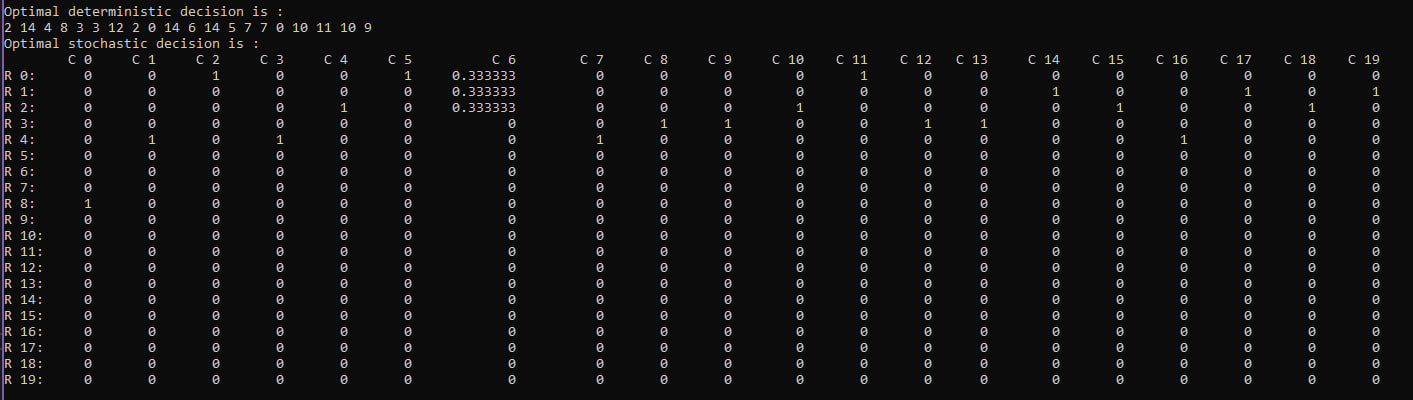
\includegraphics[width=0.5\textwidth, scale=0.2]{ReportPic/report_4.png}
    \end{minipage}
\end{figure}

Як результат роботи - видало перший ліпший $M_{i}$ (за критеріями підходить декілька)
\begin{figure}[!ht]
        \centering
        \begin{minipage}{0.55\linewidth}
            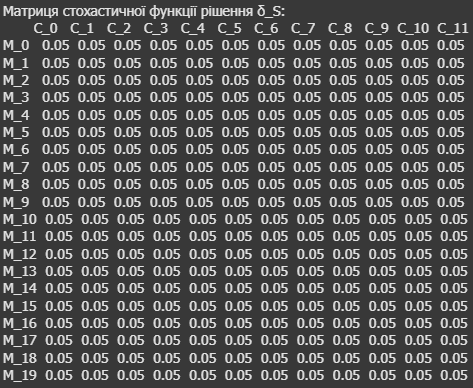
\includegraphics[width=0.8\textwidth, scale=0.6]{ReportPic/report_5.1.png}
        \end{minipage}
        \begin{minipage}{0.4\linewidth}
            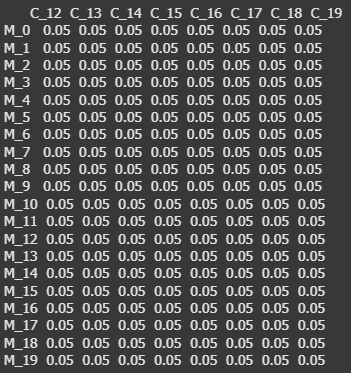
\includegraphics[width=0.8\textwidth, scale=0.5]{ReportPic/report_5.2.png}
        \end{minipage}
\end{figure}
\begin{figure}[!ht]
        \centering
        \begin{minipage}{0.55\linewidth}
            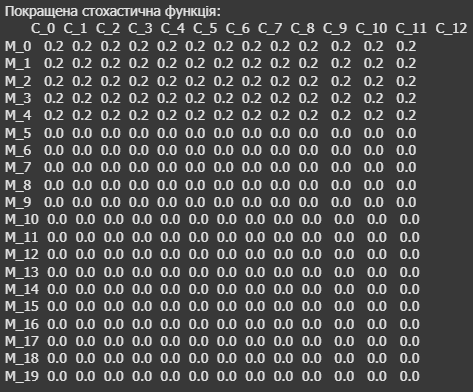
\includegraphics[width=0.8\textwidth, scale=0.6]{ReportPic/report_6.1.png}
        \end{minipage}
        \begin{minipage}{0.4\linewidth}
            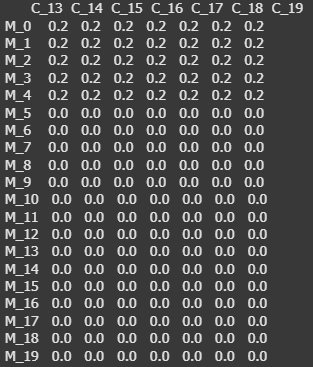
\includegraphics[width=0.8\textwidth, scale=0.5]{ReportPic/report_6.2.png}
        \end{minipage}
\end{figure}
\begin{figure}[!ht]
        \centering
        \begin{minipage}{0.85\linewidth}
            
\includegraphics[width=0.8\textwidth, scale=0.6]{ReportPic/report_7.1.png}
        \end{minipage}
        \begin{minipage}{0.85\linewidth}
            
\includegraphics[width=0.8\textwidth, scale=0.5]{ReportPic/report_7.2.png}
        \end{minipage}
\end{figure}

\section{Висновки:}
Подивившись на отримані результати середніх втрат можна впасти в ступор, оскільки вони виявилися однаковими. На нашу думку це 
може бути бути пов'язано з недостатньою точністю обрахунків. Маємо припущення, що стохастична (a.k.a. випадкова) вирішуюча 
функція мала б відповідати більшій кількості потенційних ВТ до відповідно обраного ШТ, порівняно зі строго детерміністичною. 
Вона також могла показувати як зашкально добрий результат, так і навпаки (жартуємо, будь-яку випадковість можна передбачити). 
Варто зазначити, що при збільшенні кількості вхідних даних, стохастична вирішуюча функція (яка являє собою багаторозмірну 
матрицю) буде займати багатенько пам'яті, що може сповільнити процес виконання програми.

\begin{tblr}{
    colspec={|c|*{20}{c|}},
    row{1} = {font=\bfseries}
    }
    Row & C1       & C2        & C3        & C4        & C5        & C6       & C7        & C8        & C9        & C10       & C11      & C12       & C13       & C14       & C15       & C16       & C17       & C18       & C19       & C20       \\
    0   & 0        & 0.102804  & 0.092437  & 0         & 0         & 0.111111 & 0.0894309 & 0         & 0.0728477 & 0.0956522 & 0        & 0.0814815 & 0         & 0.0748299 & 0         & 0.0791367 & 0         & 0.0541872 & 0.0956522 & 0.0894309 \\
    1   & 0        & 0         & 0         & 0         & 0.0814815 & 0        & 0.0894309 & 0.0956522 & 0.0728477 & 0.0956522 & 0        & 0.0814815 & 0         & 0         & 0.346847  & 0.0791367 & 0.0866142 & 0.0541872 & 0.0956522 & 0.0894309 \\
    2   & 0        & 0         & 0         & 0         & 0.0814815 & 0        & 0.0894309 & 0.0956522 & 0         & 0         & 0.111111 & 0         & 0.0866142 & 0.0748299 & 0         & 0.0791367 & 0         & 0.0541872 & 0.0956522 & 0.0894309 \\
    3   & 0.120879 & 0.102804  & 0.092437  & 0         & 0.0814815 & 0        & 0         & 0.0956522 & 0.0728477 & 0.0956522 & 0        & 0.0814815 & 0.0866142 & 0.0748299 & 0         & 0         & 0.0541872 & 0         & 0                     \\
    4   & 0.120879 & 0.102804  & 0         & 0.092437  & 0         & 0        & 0         & 0.0956522 & 0.0728477 & 0.0956522 & 0.111111 & 0         & 0         & 0         & 0.0990991 & 0.0791367 & 0.30315   & 0.0541872 & 0.0956522 & 0.0894309 \\
    5   & 0        & 0.0280374 & 0.0252101 & 0.0252101 & 0         & 0        & 0.0243902 & 0.026087  & 0         & 0.026087  & 0.030303 & 0.0222222 & 0         & 0.0204082 & 0         & 0.0755396 & 0.023622  & 0.0147783 & 0.026087  & 0         \\
    6   & 0        & 0.0280374 & 0.0252101 & 0.0252101 & 0.0222222 & 0.030303 & 0         & 0         & 0.0198675 & 0         & 0        & 0.0222222 & 0.023622  & 0.0204082 & 0.027027  & 0         & 0.023622  & 0         & 0         & 0.0243902 \\
    7   & 0.032967 & 0         & 0.0252101 & 0         & 0         & 0.106061 & 0.0243902 & 0         & 0.0198675 & 0         & 0.030303 & 0         & 0         & 0.0204082 & 0         & 0.0215827 & 0.023622  & 0.0147783 & 0         & 0         \\
    8   & 0.115385 & 0.0280374 & 0         & 0.0252101 & 0         & 0.030303 & 0         & 0         & 0         & 0.026087  & 0.030303 & 0.0222222 & 0.023622  & 0         & 0         & 0.0215827 & 0.023622  & 0         & 0.026087  & 0.0243902 \\
    9   & 0.032967 & 0         & 0         & 0.0252101 & 0.0222222 & 0.030303 & 0.0853659 & 0.026087  & 0.0198675 & 0         & 0.030303 & 0.0222222 & 0         & 0.0204082 & 0.027027  & 0         & 0.023622  & 0         & 0.026087  & 0.0243902 \\
    10  & 0.032967 & 0.0280374 & 0.0252101 & 0         & 0.0222222 & 0.030303 & 0.0243902 & 0         & 0.0198675 & 0.026087  & 0        & 0         & 0.023622  & 0         & 0.027027  & 0.0215827 & 0         & 0.0147783 & 0.026087  & 0         \\
    11  & 0        & 0.0280374 & 0         & 0.0252101 & 0.0222222 & 0.030303 & 0.0243902 & 0.026087  & 0.0198675 & 0.026087  & 0        & 0         & 0         & 0         & 0.027027  & 0         & 0.0826772 & 0.0147783 & 0.026087  & 0.0243902 \\
    12  & 0.032967 & 0.0981308 & 0.0252101 & 0.0252101 & 0.0222222 & 0.030303 & 0         & 0         & 0         & 0.026087  & 0        & 0.0222222 & 0         & 0         & 0.027027  & 0.0215827 & 0         & 0         & 0.026087  & 0.0243902 \\
    13  & 0.032967 & 0.0280374 & 0.0882353 & 0         & 0.0222222 & 0.030303 & 0.0243902 & 0.026087  & 0         & 0         & 0        & 0.023622  & 0         & 0.027027  & 0.0215827 & 0.023622  & 0         & 0.026087  & 0.0243902             \\
    14  & 0        & 0.0280374 & 0.0252101 & 0.0252101 & 0.0222222 & 0        & 0.0243902 & 0.026087  & 0.0198675 & 0.026087  & 0.030303 & 0.0222222 & 0.023622  & 0.0714286 & 0         & 0         & 0         & 0.026087  & 0                     \\
    15  & 0.032967 & 0.0280374 & 0.0252101 & 0         & 0         & 0        & 0         & 0.026087  & 0         & 0.026087  & 0        & 0         & 0.0204082 & 0.027027  & 0         & 0.023622  & 0         & 0.026087  & 0.0243902             \\
    16  & 0        & 0.0280374 & 0.0252101 & 0.0252101 & 0         & 0.030303 & 0.0243902 & 0.026087  & 0.0198675 & 0.026087  & 0.030303 & 0         & 0.023622  & 0         & 0.027027  & 0.0215827 & 0         & 0         & 0.0913043 & 0         \\
    17  & 0.032967 & 0         & 0         & 0.0252101 & 0         & 0.030303 & 0.0243902 & 0         & 0         & 0         & 0.030303 & 0.0222222 & 0         & 0.0204082 & 0.027027  & 0.0215827 & 0.023622  & 0         & 0.0913043 & 0.0243902 \\
    18  & 0.032967 & 0.0280374 & 0         & 0         & 0         & 0        & 0         & 0.026087  & 0.0198675 & 0         & 0.106061 & 0.0222222 & 0.023622  & 0.0714286 & 0.027027  & 0.0215827 & 0.023622  & 0.0147783 & 0         & 0         \\
    19  & 0.032967 & 0.0280374 & 0         & 0.0252101 & 0.0222222 & 0.030303 & 0.0243902 & 0.026087  & 0.0695364 & 0.026087  & 0.030303 & 0.0222222 & 0         & 0.0204082 & 0         & 0.0215827 & 0         & 0         & 0         & 0         \\
\end{tblr}